\chapter{Multi-objective optimization}
\label{sec:Metodolgia}
%\begin{refsection}

\abstract{Before tackling the problem of multiple criteria for \gls{pid} tuning, the multi-objective optimization is explained in general. First the basic formulation of the optimization problem is presented with the introduction of the Pareto front concept. The methodology chosen to solve the multi-objective optimization problem is to transform the multi-criteria situation into a single scalar cost function. However it is known that this scalarization procedure may not yield to a good Pareto front. For this reason several scalarization methods are presented and compared. The Pareto found using this scalarization methods may be used as just data that can be later used or may be directly used as part of a decision tool useful to select the final solution to the problem.} 

\section{Formalization of the multi-objective optimization problem}
\label{sec:MOOPForm}
%
A \gls{moop} arises when, in order to solve a given problem or design, it is necessary to optimize several cost functions at the same time. 

In general, these cost functions depend on the same variables and usually are in conflict.  In addition, they may be independent of one another, that is, the value of the variables that optimize one of the function do not necessarily optimize the other cost functions.

In those cases, given a set of cost functions:
\begin{equation}
\mathbf{F}(\xv)=\left[F_1(\xv), F_2(\xv), F_3(\xv), \ldots, F_k(\xv)\right]^T
\label{eq:functions}
\end{equation}
%
that depends on $n$ different variables $\xv=\left[x_1, x_2, \ldots, x_n \right]^T$, $x_i \in \mathbf{X}$, where $\mathbf{X}$ is the feasible decision space. The \gls{moop} may be formulated as follows \cite{Marler2004}:%
%
\begin{subequations}%
	\begin{align}%
	&\min_\xv \mathbf{F}(\xv), \label{eq:Min01}\\ %
	&\text{s.t.}\nonumber\\%
	& \hspace{5mm} g_j(\xv) \leq 0, \qquad j=1,2,\ldots,m  \label{eq:Min02}\\ %
	& \hspace{5mm} h_l(\xv) = 0, \qquad l=1,2,\ldots,e  \label{eq:Min03}%
	\end{align}%
	\label{eq:OptProb}%
\end{subequations}%
%
where $g_j(\xv)$ is the $j$-th inequality constraint and $h_l(\xv)$ is the $l$-th equality constraint. 
%
\subsection{Definition of the Pareto front}
In general, it is not possible to find a set of variables values that minimizes all $F$ functions. In fact, the optimization problem in \eqref{eq:OptProb} have multiple equally optimal solutions in the sense of the Pareto optimality. According to \cite{Marler2004}:
\begin{quote}
	``A point $\xv^*\in \mathbf{X}$, is Pareto optimal iff there does not exist another point, $\xv \in \mathbf{X}$, such that $\mathbf{F}(\xv)\leq\mathbf{F}(\xv^*)$, and $F_i(\xv)<F_i(\xv^*)$ for at least one function''
\end{quote}

The concept of Pareto optimality is represented in %
%
\begin{figure}[tb]
	\centering
	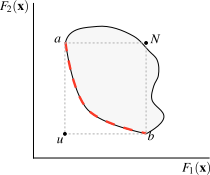
\includegraphics[width=0.8\columnwidth]{Ch5planoFun01}
	\caption{All possible solutions and the Pareto front in the function space.}
	\label{fig:planoFun01}
\end{figure}
%
figure~\ref{fig:planoFun01} for a two-function multi-objective optimization. The gray area represents the feasible function space, given by the value of $F_1(\xv)$ and $F_2(\xv)$ for all $\xv \in \mathbf{X}$. From all those points, only the points in the curve from ``a'' to ``b'' (marked with a thicker dash line) are Pareto optimal because there is not another point in the feasible decision space with a lower value of $\mathbf{F}$, but there is at least one point that has a lower value for either $F_1$ or $F_2$. The curve from ``a'' to ``b'' is the Pareto front and contains all possible solutions to problem \eqref{eq:OptProb} that are Pareto optimal. These solutions are always in the edge of the feasible function space, closer to the utopia point (the ``u'' point in the figure). The utopia point is a point in the space where all the cost functions have their minimum value. As it can be seen from figure~\ref{fig:planoFun01}, this point is more likely to be outside of the feasible function space.

Points ``a'' and ``b'' are called anchor points and represent the combination of decision variables that optimizes at least one of the functions. In this case, ``a'' is the point where function $F_1(\xv)$ has its minimum value whereas ``b'' the one in which $F_2(\xv)$ has its minimum value.

Point ``N'' is called the pseudo-nadir point, and is defined as the point with the worst values of all the anchor points.
\subsection{Different approaches to obtain the Pareto front}
To do
%----------------------------------------------------
\section{Scalarization algorithms to find the Pareto front}
\label{sec:design-methodologies}

In general, the algorithms to find the optimal value of a function are designed to be used in a single objective paradigm. In order to be able to use the same standard algorithms with a multi-objective problem, some scalarization method has to be employed.
%
\subsection{Weighted Sum}
\label{sec:WS}
\gls{ws} methodology is a popular procedure to transform a \gls{moop} into a single objective problem by creating a new objective function that is the result of the aggregation of all the functions involved with certain weight for each one \cite{Marler2004}:
%
\begin{equation}
F_{WS}(\mathbf{x}) = \sum_{i=1}^{k}\alpha_{i} {f}_{i}(\mathbf{x}),
\label{eq:JWSOriginal}
\end{equation}
%
where $\alpha_i$ is the weight of associated with function $f_i$. The idea behind the utility function $F_{WS}$ is to be able to take into account all individual cost functions at the same time. It is known that when minimizing \eqref{eq:JWSOriginal}, the solution belongs to the Pareto front. Therefore, it is of great importance to select the values of the weights that better reflect the desire of the decision-maker.

The weights have two different roles that are entangled, in one hand the weights can be used to represent the importance of one function over the others (the bigger the weight, the higher the importance) and in the other hand the weights ca be used to equalize the relative values of the functions (one function may yield higher values that shadows the others).

However, choosing the values of the weight can be difficult. In \cite{Marler2010} it is shown that the weight can be interpreted as a first order approximation of a preference function, and therefore, cannot fully take into account the desires of the decision-maker.

Lets take a two function \gls{moop} as an example. If the Pareto front wants to be computed, one may try to first normalized the function:
\begin{equation}
F_{WS}(\mathbf{x}) = \alpha_{1WS} \hat{f}_{1}(\mathbf{x}) + \alpha_{2WS} \hat{f}_{2}(\mathbf{x}),
\label{eq:JWS}
\end{equation}
with $\alpha_{1WS} + \alpha_{2WS}=1$, and $\hat{f}_{1}(\mathbf{x})$ and $\hat{f}_{2}(\mathbf{x})$ the normalized versions of $f_{1}(\mathbf{x})$ and $f_{2}(\mathbf{x})$, respectively. One possible normalization (see \cite{Marler2004}) is given by:
\begin{equation}
\hat{f}_{1}(\mathbf{x}) = \frac{f_{1}(\mathbf{x})-\min{\left( f_{1}(\mathbf{x})\right) }}{\max{(f_{1}(\mathbf{x}))}-\min{\left( f_{1}(\mathbf{x})\right) }}.
\label{eq:NormalizedJ}
\end{equation}

With this normalization, the utopia point is moved to the origin and the maximum value of the new normalized function is 1.

The optimization problem then is written as:
\begin{equation}
\begin{gathered}
\min_{\mathbf{x}}{\; F_{WS}(\mathbf{x})}, \\
\text{s.t.} \; h(\mathbf{x})=0, \\
g(\mathbf{x}) \leq 0,
\end{gathered}
\label{eq:WSProblem}
\end{equation}
%
where $h(\mathbf{x})$ and $g(\mathbf{x})$ are the equality and inequality constraints of the original problem. To find the Pareto front, the problem in \eqref{eq:WSProblem} is solve varying the weights. However, it is known that the \gls{ws} method is not appropriate to find the Pareto front. In first place, when \eqref{eq:JWS} is minimized for different values of $\alpha_{1WS}$ and $\alpha_{2WS}$ in order to obtain the Pareto front, an even distribution of the weights does not assure an even distribution of the points in the front. Also, with \gls{ws} it is not possible to obtain Pareto points in the non-convex region of the front, and therefore, not all the possible solutions can be found \cite{Das1997}. In order to tackle this issue, alternative problem formulation have been proposed in the literature to obtain the Pareto front which are presented next.
%--------------------------------------------------
%--------------------------------------------------
\subsection{Normal Boundary Intersection}
\label{sec:NBI}
%
The \gls{nbi} is a variation in the way that the \gls{moop} is posed as a single objective optimization problem, in order to obtain an even spaced Pareto front \cite{Das1998}. In %
%
\begin{figure}[b]%
	\centering
	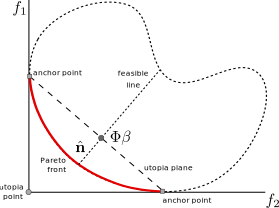
\includegraphics[width=0.8\columnwidth]{Ch5NBI}%
	\caption{\gls{nbi} optimization method.}%
	\label{fig:NBI}%
\end{figure}
%
figure~\ref{fig:NBI}, a representation of the method is shown for two normalized objective functions. If the utopia plane (the plane that contains the anchor points, in the case of a bi-objective problem, the straight line that joins the anchor points) is parameterized by $\Phi\mathbf{\beta}$, where $\Phi(:,i)=\mathbf{F}(\mathbf{x}_i^*)-\mathbf{F}(\mathbf{x}^*)$, $\mathbf{F}(\mathbf{x}_i^*)$ is the value of the multi-objective function evaluated in the $i$th anchor point, $\mathbf{F}(\mathbf{x}^*)$ is the value of the function at the utopia point, and $\beta$ is chosen as:
\begin{equation}
\beta=
\left[\begin{tabular}{c}
$\alpha_{1NBI}$ \\ $\alpha_{2NBI}$
\end{tabular}\right],
\label{eq:Beta}
\end{equation}
with $\alpha_{1NBI}+\alpha_{2NBI}=1$.

The central idea behind the \gls{nbi} method is to find the maximum distance from the utopia plane towards the utopia point (with direction $\hat{\mathbf{n}}$) that is normal (or quasi normal as proposed in \cite{Das1998}) to the utopia plane. In other words, this method finds the border of the feasible region that is closer to the utopia point (farther from the utopia plane). This problem is considered a subproblem, because with one given $\beta$,only one point of the Pareto front is found but, by varying this parameter $\beta$ evenly, it is possible to obtain an even spaced realization of the front.

The problem then is posed as follows:%
%
\begin{equation}
\begin{gathered}
\max_{\xv,v}{\;v}, \\
\text{s.t.} \ \Phi \boldsymbol{\beta} + v \hat{\mathbf{n}} = \mathbf{F}(\xv),\\
h(\xv)=0, \\
g(\xv) \leq 0.
\end{gathered}
\label{eq:NBIProblem}
\end{equation}%

The \gls{nbi} method converts the original problem by adding an equality constraint. By maximizing the new variable $v$ (which represents the distance from the utopia plane towards the utopia point), the front that is closer to the utopia point is found. An alternative formulation of \eqref{eq:NBIProblem} was proposed in \cite{Shukla2007} to ensure that only the points that really belongs to the Pareto front are found.

This method has been widely used in several areas.For example, in \cite{Stehr2003} was used to analyze the compromise between gain and phase margin when designing analog circuits. In \cite{Sendin2004}, the \gls{nbi} was considered in the design of nonlinear bioprocesses. In \cite{Ierapetritou2007a} the \gls{nbi} is used to optimize the scheduling of a chemical process with uncertainty. In \cite{Vahidinasab2010} \gls{nbi} is applied to develop optimal bidding strategies for the participants of oligopolistic energy markets; the social welfare and the emissions are considered as the cost functions and the constraints take into account the characteristics of the generators and the power flow of the system. In \cite{Ganesan2013}, \gls{nbi} is used in conjunction with a meta-heuristic algorithm to generate optimal solution options to the green sand mould system problem. In \cite{Brito2014} the method is used coupled with mean-squared error functions in a robust parameter design of the surface roughness in end milling process. In \cite{Rubio-Largo2014} the method is adapted to solve a traffic grooming problem in the telecommunication field. In \cite{Rojas2015b} a comparison between several scalarization methods, including \gls{nbi}, was presented for a \gls{foptd} plant where different disturbance sources are considered. In \cite{Naves2017} \gls{nbi} is used for the optimization of methyl orange treatment with ozone. In \cite{Simab2018} a model for short-term hydrothermal scheduling problem in the presence of the pumped-storage technology and stated as Mixed-Integer Non-Linear Programming, while the scalarization was done using \gls{nbi}. Finally, in \cite{Moura2018} \gls{nbi} was used in the construction of a Pareto boundary chart of a treatment of a synthetic solution of amoxicillin in a reactor with ozone bubbling.
%-------------------------------------------------- 
\subsection{Normalized Normal Constraint}
\label{sec:NNC}
The \gls{nnc} is presented in \cite{Messac2003} and is intended to improve the results of the \gls{nbi} by formulating the optimization problem only with inequality constraints and by filtering all the non-Pareto optimal points. The main idea of the methodology is presented in
%
\begin{figure}[b]%
	\centering
	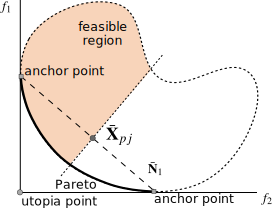
\includegraphics[width=0.8\columnwidth]{Ch5NNC}%
	\caption{NNC optimization method.}%
	\label{fig:NNC}%
\end{figure}
%
figure~\ref{fig:NNC}: the utopia plane is parameterized in a similar way as the \gls{nbi} but, instead of constraining the points to be within a line, the new constrained feasible region is constructed with the original feasible region and a line that is normal to the utopia plane. With this new feasible region it is only required to minimize one of the functions (e.g. $f_{1}$) in order to find the Pareto front.

By varying the parameter $\bar{\mathbf{X}}_{pj}$ along the utopia plane, it is possible to find an even spaced front. $\bar{\mathbf{X}}_{pj}$ is computed as%
%
\begin{equation}
\bar{\mathbf{X}}_{pj}= \alpha_{1NNC} \mathbf{\hat{F}}(\mathbf{x}_1^*)+\alpha_{2NNC} \mathbf{\hat{F}}(\mathbf{x}_2^*).
\label{eq:Xpj}
\end{equation}%
%
with $\alpha_{1NNC}+\alpha_{2NNC}=1$ and where $\mathbf{\hat{F}}(\mathbf{x}_1^*)$ is the first anchor point and $\mathbf{\hat{F}}(\mathbf{x}_2^*)$ is the second. The methodology can be extended to higher dimensions.

The optimization problem can be written as follows:
%
\begin{equation}
\begin{gathered}
\min_{\mathbf{x}}{\; \hat{f}_{1}(\mathbf{x})}, \\
\text{s.t.} \ \bar{\mathbf{N}}_1^T \left(\hat{\mathbf{F}}(\mathbf{x})-\bar{\mathbf{X}}_{pj}\right) \leq 0,\\
h(\mathbf{x})=0, \\
g(\mathbf{x}) \leq 0,
\end{gathered}
\label{eq:NNCProblem}
\end{equation}
%
where $\bar{\mathbf{N}}_1$ is the vector that contains the direction of the utopia plane. In some cases, the optimization may yield points that do not belong to the Pareto front. In \cite{Messac2003}, the authors propose to use a filter algorithm to eliminate those points.

This method has been used in several cases. Also in \cite{Hosseini2016a} the method was implemented to optimally solve the transmission congestion management taking into account the cost of congestion management, voltage stability margin, and transient stability margin. In \cite{Sanchez2017a}, the \gls{nnc} was considered to find optimally balanced tuning rules for fractional-order proportional-integral-derivative controllers for \gls{foptd} process models subject to a robustness constraint. In \cite{Mittal2017a} the NNC was used in conjunction with an evolutionary algorithm to find the optimum number and location of wind turbines in a wind farm. In \cite{Benki2018}, the \gls{nnc} was implemented in the design of an aerosol can, tanking into account both the dome growth and the dome reversal pressure DRP. In \cite{Tan2018a}, the \gls{nnc} was applied in the design of microvascular panels for battery cooling applications. The NNC is also applied in \cite{Liu2019} within their algorithm to optimally control the glycerol in a 1,3-propanediol batch process.

\subsection{Enhanced Normalized Normal Constraint}
\label{sec:ENNC}
The \gls{ennc} \cite{Sanchis2008}, is a new perspective of the original \gls{nnc} method. Implicitly, the \gls{nnc} method supposes that in each anchor point, the other functions that are not optimal, have their worst value. For a two functions optimization, this is always the case; however for more than two functions this supposition is not true in general. The \gls{ennc} method redefines the anchor points in such a way that the supposition of the \gls{nnc} holds true, and then the same method may be used. Other advantage of the \gls{ennc} is that it is possible to expand the explored regions of the problem, given a better representation of the Pareto front.
%
The new anchor points (called pseudo anchor points) are defined as:
\begin{equation}
F_i^{**} = \left[
\begin{tabular}{cccccc}
$f_1^N$ & $f_2^N$ & $\cdots$ & $f_i^{*}$ & $\cdots$ & $f_n^N$
\end{tabular}
\right],
\label{eq:PseudoAnchor}
\end{equation}
%
where $f_i^N$ if the value of function $f_i$ at the pseudo nadir point. The effect of this new definition is to enlarge the utopia hyper plane and scaling the functions in such a way that the Pareto front is evenly obtained while the unexplored regions of the Pareto are reduced.

The Pareto is then computed using the same methodology as in the \gls{nnc} case. This method has also been applied in several cases, for example in \cite{Contreras-Leiva2016}, the \gls{ennc} is applied in the optimization of the tuning parameters of a \gls{2dof} \gls{pid} controller for an \gls{soptd} plant. In\cite{Pereira2017b} an augmented version of the \gls{ennc} is applied to optimized the milling process of aluminum alloy Al 7075 taking into account the axial cutting force, the energy consumption and the material removal rate. The \gls{ennc} is tested in the optimization of a multiobjective model based predictive controller and compared with different techniques in \cite{Toro2011} and for the nonlinear case in \cite{Vallerio2014}.
%--------------------------------------------------
\section{Solution selection from the Pareto front}
\label{sec:Selection}
%%--------------------------------------------------------------------------
%%-------------------------------o-o-o--------------------------------------
%%--------------------------------------------------------------------------
The optimizations techniques presented in Section~\ref{sec:design-methodologies} are very well suited to find the Pareto Front of a multiobjective optimization problem. However, in the end, it is necessary to decide which of the multiple equally optimal points is the one that is going to be selected as the final solution.

Consider the general Pareto Front presented in 
\begin{figure}[b]
	\centering
	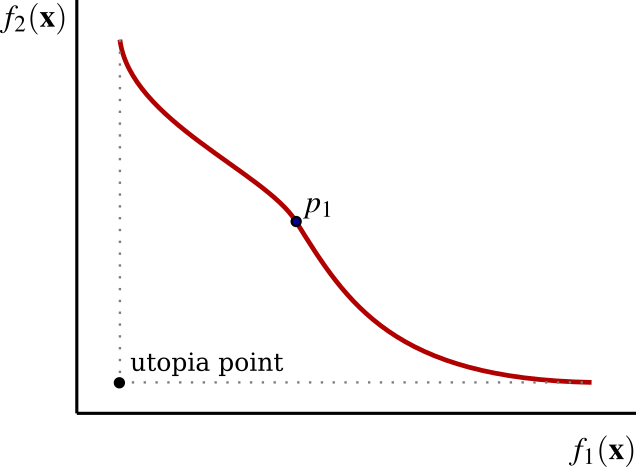
\includegraphics[width=0.8\columnwidth]{Ch5GeneralPareto}
	\caption{General Pareto Front with one solution selected.}
	\label{fig:Ch5GeneralPareto}
\end{figure}
%
Figure~\ref{fig:Ch5GeneralPareto}. Once the Pareto is computed, it is certainly very useful to plot it to see how the cost functions $f_1(\mathbf{x})$ and $f_2(\mathbf{x})$ vary with the change in the decision variables $\mathbf{x}$. In this figure, the arbitrary solution $p_1$ is pointed out. By definition, all points in the Pareto Front are equally optimal, therefore, what makes $p_1$ any special from other points? More important, how any of the Pareto points can be selected from any other?

One may then conclude that obtaining the Pareto front is half the solution to the \gls{moop}. The final task to fully solve the problem is to be able to select one of the (maybe infinite) possible points of the Pareto. With a front like the one presented in Figure~\ref{fig:Ch5GeneralPareto}, it may be easy to explore all possible solutions, but with more than three objective functions, it is impossible to directly plot the front. And even with three objectives, the visualization of the results may be cumbersome.

Even more, the plot of Figure~\ref{fig:Ch5GeneralPareto} contains the solutions viewed from the function space, but what is really necessary is to know the value of the decision variables. But each of every point in the Pareto is associated with a $n$-size vector representing one of the optimal solutions. Once again, plotting the Pareto is not enough to help the decision maker to solve the problem.

For these reasons, once the Pareto is found, it may be useful to accomplish some tasks to help the decision maker:
\begin{itemize}
	\item  Visualize the Pareto to understand the relation between the cost functions and the decision variables.
	\item Use the Pareto as data for the construction of a decision tool.
	\item Use the Pareto as part of a decision tool.
\end{itemize}
In the following, these three tasks are going to be explored.
%
\subsection{Visualization of the Pareto Front}
\label{sec:ParetoVisualization}
%
One of the advantages of using a multiobjective problem approach, is its ability to take into account many cost functions at the same time, and being able to find the set of the \emph{best} solutions. This is the ultimate goal of a multiobjective optimisation, to provide useful information to the decision makers in order to help to choose according to its preferences. This can be done in terms of a large set of raw data that has lately to be processed accordingly. This introduces some cognitive issues that become harder and a clear obstacle for decision making stage, especially when having many objectives (say more than 3). Although there are some performance metrics that can evaluate the quality of a Pareto front approximation set (Inverted Generational Distance \cite{Bosman2003} and Hypervolume \cite{Zitzler1999} among others), it is still not intuitive this approach really helps the decision maker to understand the trade-off relationship among objectives.

In contrast, high-dimensional data visualisation is a widely recognised effective way to facilitate the analysis and understanding of multidimensional data. more effective and intuitive to facilitate the decision maker stage to understand the trade-off solutions and thus make a meaningful decision. In the context of multi-objective optimisation, comparing to quantitative performance metrics, visualisation is, in principle, able to provide a decision maker better insights about Pareto front approximation sets (e.g. the distribution of solutions, the geometric characteristics of Pareto front approximation) thus to facilitate the decision-making (e.g. the exploration of trade-off relationship, the knee region or region of interest).

According to \cite{Gao2019} a high quality visualisation tool must provide three types of information in the high dimensional space. 
\begin{itemize}
\item  Should provide accurate shape, location, and range of the approximate Pareto front. 
\item  From the provided visualisation, decision makers can observe trade-off between objectives, monitor the evolution progress, assess the quality of the approximate front, and select their preferred solutions if desired. 
\item  Should be scalable to any dimensions, handle a large number of individuals on the approximate front, and simultaneously visualise multiple fronts for the purpose of visual comparison. Moreover, the resulted visualisation plot should be robust and insensitive to the addition or removal of an individual.
\end{itemize}

To tackle these issues, different kinds of plots have been proposed in the literature that tries to present all the information of the Pareto in a bi-dimensional graph. Generally speaking, they can be divided into three categories. Interested readers are encouraged to ?nd a recent taxonomy from \cite{B.2018}.

\begin{description}
\item [A. Visualisation of All Objective Information] These visualisation techniques aim to reveal all individual objective information of the underlying approximation set. Specifically, scatter plot is the most commonly utilised data visualisation technique that provides a holistic exploration of the population distribution. 

\item [B. Visualisation via Dimension Reduction] Techniques in this category aims to transform the high-dimensional data into a lower dimensional space to facilitate the human cognition. In modern data analytics, there are many dimension reduction techniques available to implement such transformation.  Instead of using dimension reduction techniques from machine learning, In \cite{Blasco2008}, Blasco et al. proposed a new visualisation technique called level diagrams to visualise the approximation set in a objective-wise manner. More specifically, each diagram is a two-dimensional scatter plot where the horizontal coordinate represents the objective value at the corresponding objective while the vertical coordinate indicates the distance with respect to the ideal point. As claimed by the authors, the level diagrams are able to facilitate the investigation of some of the Pareto front characteristics, i.e. discontinuities, closeness to ideal point and ranges of attainable values. 

\item [C. Visualisation via a Transformed Coordinate System] Techniques in this category share some similarity with the dimension reduction. They also aim to visualise the original high-dimensional data in a lower-dimensional space. But they try to maintain the original information as much as possible. For example, Ibrahim et al. \cite{Ibrahim2016} developed a variant of the classic Radial coordinate visualisation (RadViz) \cite{Hoffman2002}, called 3D-RadViz, by adding an additional dimension. In particular, this additional dimension represents the perpendicular distance between a solution and a hyper-plane formed by the extreme points of the underlying population. By doing so, the 3D-RadViz is able to provide the information of the convergence of the population. 
\end{description}

As usual when there do exist different approaches to deal with a complex problem, there is  no single visualisation technique is able to provide a comprehensive understanding of the characteristics of the approximation set. It is important to know the specific characteristics, pros and cons of each approach and evaluate the suitability for the problem at hand.
  
\subsection{The Pareto as data for the construction of a decision tool}
\label{sec:ParetoData}
%
Since the Pareto front cannot be considered as the final solution of the \gls{moop}, one may use it as the basis to construct a tool that takes advantage of the multiple optimal points found.

In other words, the Pareto front becomes the raw material that is used to produce the final decision tool. This tool may be an algorithm (as a tuning rule for PID controllers for example) that incorporates the information obtained from the optimization to produce a final decision.

For example in \cite{Zhao2007}	the concept of Pareto optimality is used to define a genetic programming approach for optimal decision trees. The author presented a Java code for the final tool and use code in two different study cases.

Another example can be found in \cite{Das2012}. In this paper, the route for the transportation of hardzarous waste has to be selected taking into account the cost of the route and the mortality and morbidity of incidents. Once the Pareto frontier has been obtained, the authors present a selection criteria where the Cost Elasticity of risk and the Knees on the Pareto are taken into account for the final decision.



\subsection{The Pareto Front as part of a decision tool}
\label{sec:ParetoDecision}
\textbf{To do}



















%\printbibliography
%\end{refsection}